\chapter{4}
\label{ch:4}

\todo{Name chapter}

\section{Methodology}
We decided to analyze the arXiv and PubMed Central corpora as a representative sample of scholarly publications across Science, Technology, Engineering, and Math (STEM) disciplines, in order to understand how scholarly code is being referenced over time and, therefore, both woven into the fabric of our scholarly conversation and worthy of preservation. arXiv is one of the largest and most popular pre-print services, and the corpus contains over 2 million submissions \cite{fromme-cornell2022} from eight disciplines: physics, mathematics, computer science, quantitative biology, quantitative finance, statistics, electrical engineering and systems science, and economics. The arXiv corpus does not allow for anonymous submissions, is publicly available, and is accessible for programmatic acquisition and analysis. The PubMed Central (PMC) corpus contains publicly available full-text articles from a wide range of biomedical and life sciences journals. Only peer-reviewed journals are eligible for inclusion.\footnote{https://www.ncbi.nlm.nih.gov/pmc/pub/addjournal/} The most prevalent journals in the corpus are listed in Table \ref{tab:pmc_corpus} along with the number of articles in the corpus, the date of the first article available, and the date of the latest article. The size and availability of the arXiv and PMC corpora make them suitable for the purposes of our study.  

\begin{table}
  \centering
  \begin{tabular}{|l|r|r|r|}
    \hline
    Journal & Articles & Earliest & Latest\\
    \hline
    The Indian Medical Gazelle & 29,143 & 1866 & 1955\\
    The Journal of Cell Biology & 24,349 & 1962 & 2022\\
    The Journal of Experimental Medicine & 24,207 & 1896 & 2022\\
    BMJ Open & 21,565 & 2011 & 2022 \\
    Edinburg Medical Journal & 20,160 & 1855 & 1954\\
  \hline
\end{tabular}
\caption{Five most popular journals in the PMC corpus}
\label{tab:pmc_corpus}
\end{table}

In April 2007, the arXiv identifier scheme changed to accommodate a larger number of submissions and to address other categorization issues.\footnote{https://arxiv.org/help/arxiv\_identifier} We decided that beginning our arXiv corpus in April 2007 would suit our analysis, because three of the four repository platforms that we analyzed began after 2007. Each pre-print in arXiv can have multiple versions. When an author uploads a new version of the pre-print to the service, the version number increments by one. All versions of a pre-print are accessible in arXiv via a version-specific URI. For our analysis, we considered only the latest version of each submission, assuming that the final submission was the most complete and most representative of the author's intentions. With only the latest version of each submission, our arXiv corpus contained 1.56 million publications in PDF format from April 2007 to December 2021. 

The PMC corpus includes articles from the late 1700s to present. In order to more easily compare the corpora and because, as previously noted, three of the four repository platforms we analyzed began after 2007, we decided that beginning our PMC corpus in January 2007 was appropriate for our analysis. Additionally, the PMC corpus  separates articles that are available for commercial use from those that are only available for non-commercial use. We chose to analyze the articles that were only available for non-commercial use. Our PMC corpus contained 1.08 million publications in PDF format from 2007 to 2021. Between the arXiv and PMC corpora, we analyzed 2,641,041 publications. 

A study by Milliken \cite{iasge_enviro_scan} conducted initial testing of GitHub, GitLab, SourceForge, and Bitbucket to understand the archival quality available through Brozzler (Archive-It's crawler), a Standard crawler (Heritrix and Umbra), and Memento Tracer. Our project is a continuation of that study and, as a result, we chose to analyze the use of those four GHPs in the arXiv and PMC corpora. The GHPs are summarized in Table \ref{tab:repos}.

\begin{table}
  \centering
  \begin{tabular}{|l|r|l|l|}
    \hline
    Name & Start Date & Protocol & URI\\
    \hline
    SourceForge & 1999 & git and SVN & \url{https://sourceforge.net}\\
    Bitbucket & 2008 & git & \url{https://bitbucket.org}\\
    GitHub & 2008 & git & \url{https://github.com}\\
    GitLab & 2014 & git & \url{https://gitlab.com}\\
  \hline
\end{tabular}
\caption{Repository Platforms}
\label{tab:repos}
\end{table}

URIs are not exclusively found in the References section of a publication; they also commonly appear in footnotes and the body of the text. To extract all of the URIs in each publication, regardless of location, we leveraged two Python libraries: PyPDF2\footnote{https://pypi.org/project/PyPDF2/} and PyPDFium2.\footnote{https://pypi.org/project/pypdfium2/} We used PyPDF2 to extract annotated URIs and PyPDFium2 to extract URIs from the PDF text. We followed a similar URI characterization method as that done by Klein et al. \cite{klein-plos2014} who identified URIs to ``Web at large" resources in-scope for their study. Since we are investigating links to GHPs, our primary goal with extraction was to identify URIs to one of the four GHPs. However, we also identified URIs to the Web at large to provide context for the frequency and use of URIs to the GHPs. To do this, we filtered out a number of URIs that were out of scope for this study. We dismissed URIs with a scheme other than HTTP or HTTPS, including localhost and private/protected IP ranges. We also dismissed URIs to arXiv, Elsevier RefHub,\footnote{https://refhub.elsevier.com} CrossRef Crossmark \cite{hendricks-crossref-2020}, and HTTP DOIs and, as such, follow the definition of URIs to ``Web at large" resources that are in-scope for our work. DOIs resolve to artifacts, most commonly papers but increasingly also to data (e.g., via Dryad) and source code (e.g., via Zenodo). Links to Elsevier RefHub and CrossRef Crossmark function similarly to DOIs and are often added by the publisher. We decided to exclude DOI and DOI-like references following Klein et al.'s assumption that, for the most part, such artifacts are in-scope for existing archiving and preservation efforts such as LOCKSS \cite{reich-dlib2001}, CLOCKSS \cite{reich-serials2008}, and Portico \cite{fenton-serials2006}. Our source code is available on GitHub \cite{Extract-URLs}.

After extracting URIs from the PDFs in our corpora, we found 7,746,682 in-scope URIs: 4,039,772 URIs from the arXiv corpus and 3,706,910 URIs from the PMC corpus. Out of 2.64 million files, 1,439,177 files ($54.06\%$) contained a URI. Once we had collected all of the URIs from the PDFs, we used regular expressions to filter and categorize the URIs that referenced one of the four GHPs. As a result, URIs to repository pages with custom domain names \cite{custom-domain} were not captured. We found a total of 253,590 URIs to one of the four GHPs: 231,206 URIs from the arXiv corpus and 22,384 URIs from the PMC corpus. All GHP URIs in a publication have been deemed by the authors to be important enough for inclusion in the publication. As a result, we do not differentiate links to GHPs regardless of link depth or location in the publication. Inclusion of a GHP URI does not indicate an authorship or ownership claim. GHP URIs in a publication indicate that a resource either 1) impacted the work presented in the publications or 2) was a product of the study. Both cases communicate the importance of the repository and need for preservation. The number of URIs for each GHP are shown in Table \ref{tab:repo_count}. The URIs to GitHub account for 92.3\% of the URIs to one of the four GHPs. 

\begin{lstlisting}[caption={Regular expressions to sort URLs to repositories in GitHub, GitLab, SourceForge, and Bitbucket from all other URLs}, label={lst:regex}]
  sf = re.search(r"(sourceforge.net)", url)
  if sf is not None:
    if re.search(r"(?=("+'|'.join(sf_sitemap)+r"))", url) is not None:
      # URL included in the SourceForge sitemap
    else:
      # SourceForge repository URL

  gh = re.search(r"(github.com|github.io)", url)
  if gh is not None:
    if re.match(r'com,github,gist', url):
      # URL to Gist
    elif re.match(r'org,archive,web\)\/save\/', url):
      # URL to Internet Archive
    elif re.match(r'org,archive,web\)\/web\/', url):
      # URL to Internet Archive
    elif re.match(r'io,github', url):
      # URL to GitHub.io
    elif not re.match(r"^(https?:\/\/w{0,3}.?github.com\/.+)", url) or re.search(r"(?=("+'|'.join(gh_sitemap)+r"))", url) is not None:
      # URL included in GitHub sitemap and old GitHub pages URL formats
    else:
      # GitHub repository URL
  
  gl = re.search(r"(gitlab.com|gitlab.io)", url)
  if gl is not None:
    if re.match(r'io,gitlab', s):
      # URL to GitLab.io 
    elif not re.match(r"^(https?:\/\/w{0,3}.?gitlab.com\/.+)", url) or re.search(r"(?=("+'|'.join(gl_sitemap)+r"))", url) is not None:
      # URL included in GitLab sitemap and old GitLab pages URL formats
    else:
      # GitLab repository URL
  
  bb = re.search(r"(bitbucket.org|bitbucket.io)", url)
  if bb is not None:
    # is it a link to a repo?
    if not re.match(r"^https?:\/\/(w{0,3}.?bitbucket.org\/.+|.*@bitbucket.org\/.+)", url) or re.search(r"(?=("+'|'.join(bb_sitemap)+r"))", url) is not None:
      # is it a link to Bitbucket pages?
      if re.match(r"^https?:\/\/((?!www).*.?bitbucket.org|.*bitbucket.io)", url):
        # URL to Bitbucket pages
      else:
        # Non-repository Bitbucket URL
    else:
      # Bitbucket repository URL
\end{lstlisting}

\begin{table}
    \centering
    \begin{tabular}{|l|r|r|}
    \hline
    Repository Platform & arXiv & PMC\\
    \hline
    GitHub & 215,621 & 18,471\\
    SourceForge & 9,412 & 3,309\\
    Bitbucket & 3,525 & 437\\
    GitLab & 2,648 & 167\\
  \hline
    \end{tabular}
    \caption{Number of references to each GHP in the arXiv and PMC corpora}
    \label{tab:repo_count}
\end{table}

\section{Results}
By extracting URIs for the four repository platforms, we made a number of interesting observations. As shown in Figure \ref{fig:combo_urls}, we found a continuation of the significant increase in the prevalence of URIs in publications that Klein et al. \cite{klein-plos2014} found in 2014. Figure \ref{fig:combo_urls} shows the average number of in-scope URIs and the average number of URIs to one of the four GHPs in each publication by month of submission for both the arXiv and PMC corpora. The URIs to one of the four GHPs are a subset of in-scope URIs extracted from the publications. From 2007 to 2021, the average number of URIs per publications has steadily risen. In 2007, publications contained an average of 1.02 URIs. In 2021, publications contained an average of 5.06 URIs. The average number of in-scope URIs in each publication is indicated by the red and orange lines in Figure \ref{fig:combo_urls}. 

\begin{figure}
    \centering
    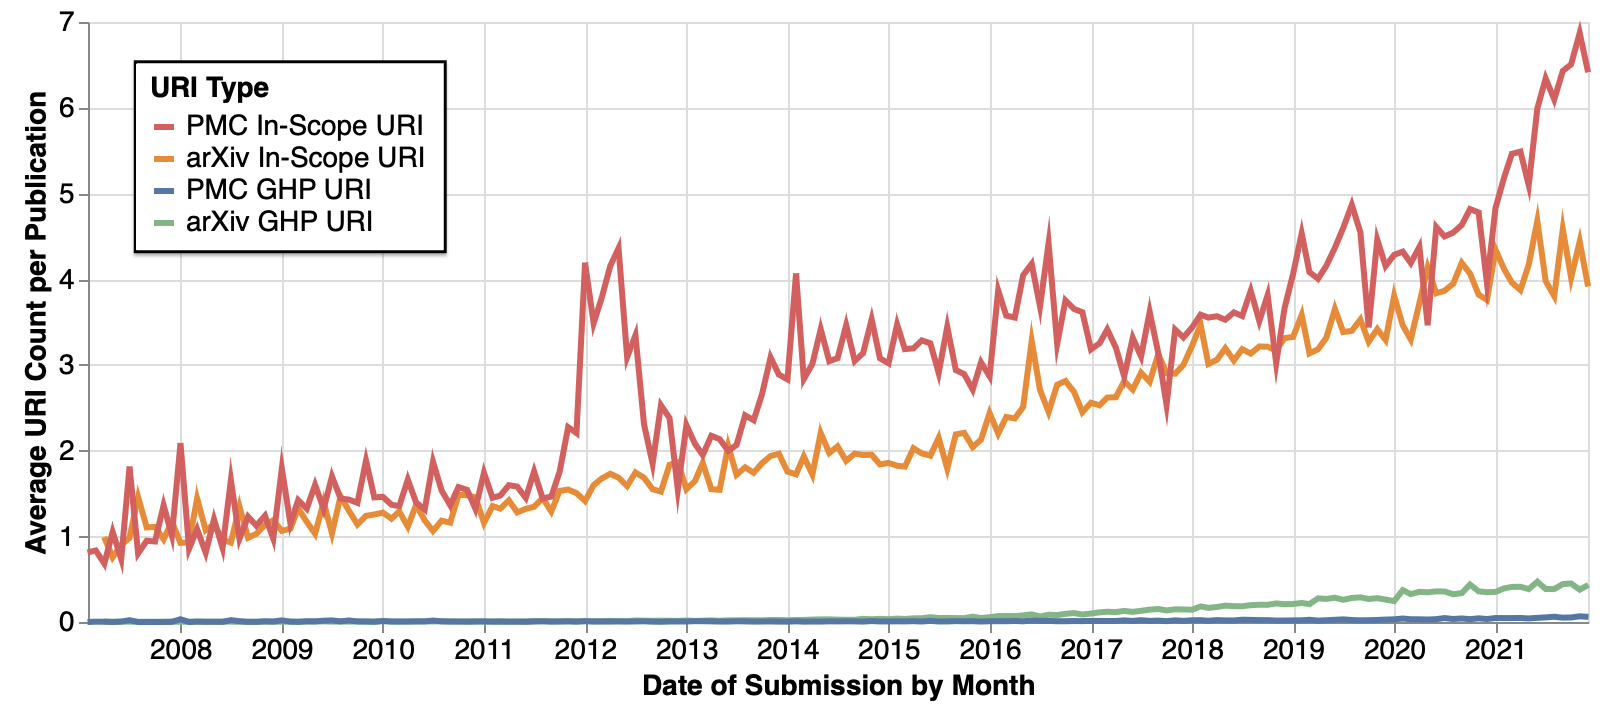
\includegraphics[width=\linewidth]{combo_urls_over_time.png}
    \caption{The average number of in-scope URIs and URIs to repository platforms per publication over time}
    \label{fig:combo_urls}
\end{figure}

While the prevalence of URIs in general has increased, the number of URIs to repository platforms has also grown from 2007 to 2021. Just as there was a shift from not including Web resources in scholarly publications to including Web resources, there has also been a shift to referencing repository platforms in scholarly publications. Figure \ref{fig:repo_urls} shows that references to GitHub have steadily risen from 2014 to 2021 while the frequency of references to the other three platforms have remained low during that time period. In the arXiv corpus shown in Figure \ref{fig:arxiv_repo_urls}, less than 1\% of publications contain a URI to GitLab, Bitbucket, or SourceForge in any given year from 2007 to 2021. However, an average of 20\% of publications contained a URI to GitHub in 2021. The PMC corpus in Figure \ref{fig:pmc_repo_urls} shows an initial prevalence of SourceForge beginning in 2007, but it is replaced by GitHub in 2015. Both graphs show a steady increase in the use of GitHub URIs in scholarly publications. Like URIs to the Web at large, URIs to repositories contribute to the context and argument of the publication. As the prevalence of GitHub URIs in publications increases, so does the importance of archiving source code repositories with its scholarly ephemera.

\begin{figure}[h]
\centering
\begin{subfigure}{\textwidth}
    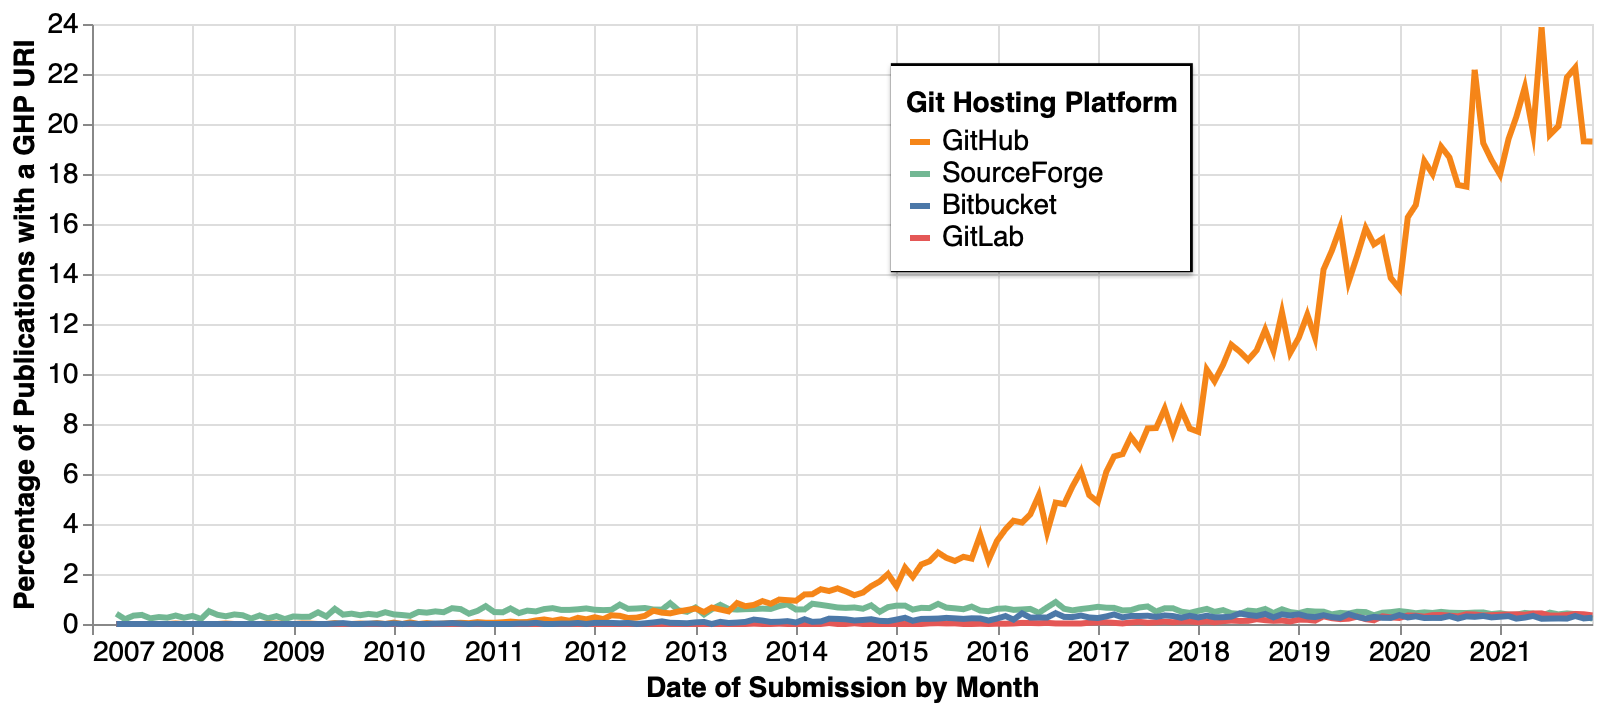
\includegraphics[width=\textwidth]{arxiv_repo_urls.png}
    \caption{arXiv corpus}
    \label{fig:arxiv_repo_urls}
\end{subfigure}
\hfill
\begin{subfigure}{\textwidth}
    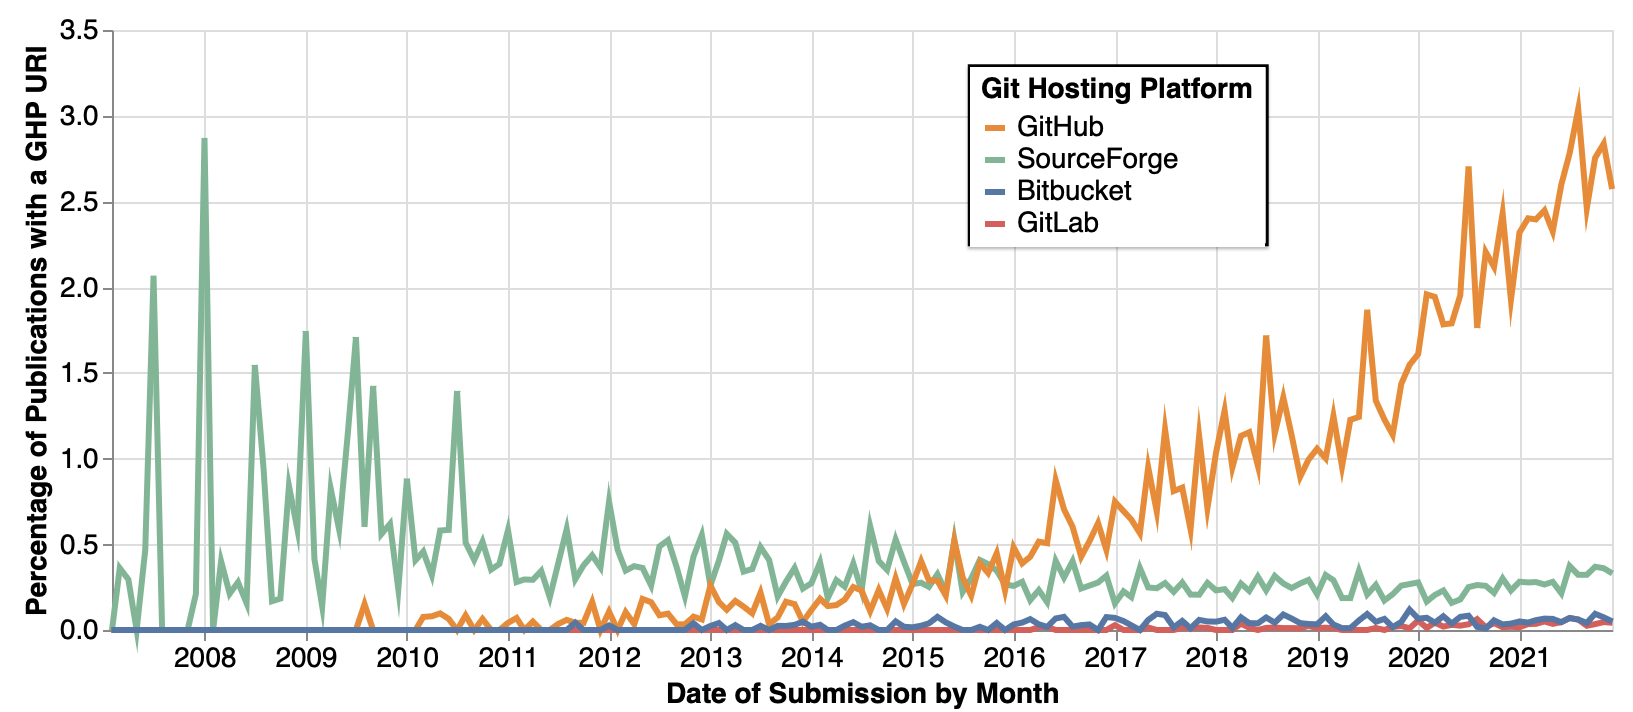
\includegraphics[width=\textwidth]{pmc_repo_urls.png}
    \caption{PMC corpus}
    \label{fig:pmc_repo_urls}
\end{subfigure}
        
\caption{The percentage of publications with a URI to a repository platform over time. Please note that the graphs are not on the same y-axis scale.}
\label{fig:repo_urls}
\end{figure}

Additionally, while 67\% of publications only reference a given repository once, 45,780 publications reference a given platform's holding more than once. Figure \ref{fig:ccdf} shows the frequency of GHP URIs in publications that contain one or more GHP URI. For example, as shown in Figure \ref{fig:arxiv_ccdf}, of the 125,711 publications in the arXiv corpus that reference GitHub, 83,328 publications ($66.3\%$) reference GitHub once, 42,383 publications ($33.7\%$) reference GitHub more than once, and 863 publications ($0.687\%$) reference GitHub more than ten times. We manually inspected a sample of the publications with the most URIs to one of the four GHPs and found these publications tend to detail a software product or provide an overview of a topic, such as survey paper. The top three publications containing the most URIs to a GHP include 153 \cite{dhole-arxiv2021}, 160 \cite{agol-arxiv2021}, and 896 \cite{truyen-arxiv2021} URIs to GitHub. Dhole et al. \cite{dhole-arxiv2021} developed a software product and included URIs to the implementation of the features listed in the publication. Agol et al. \cite{agol-arxiv2021} created an open-source package and linked to the implementation of the algorithms and processes described in the publication. Truyen et al. \cite{truyen-arxiv2021} wrote a survey paper comparing frameworks. A majority of the frameworks surveyed are documented in GitHub, so the survey contains numerous URIs to the documentation. The publication by Truyen et al. with 896 URIs to GitHub is not included in Figure \ref{fig:ccdf}, because it represents such a large outlier compared to the other publications in the corpus.

As shown in Figure \ref{fig:pmc_ccdf}, of the 11,386 publications in the PMC corpus that reference GitHub, 7,983 publications ($70.1\%$) reference GitHub once, but 3,403 publications ($29.9\%$) reference GitHub more than once and 60 publications ($0.527\%$) reference GitHub more than ten times. The top four publications with the most URIs to a GHPs contain 39 \cite{kuo-pmc2019,kayani-pmc2021}, 40 \cite{chen-pmc2021}, and 45 \cite{yang-pmc2021} URIs to GitHub. Like the arXiv corpus, each of these four publications provides a survey of the computation tools available in a given discipline.

\begin{figure}[htbp]
\centering
\begin{subfigure}{\textwidth}
    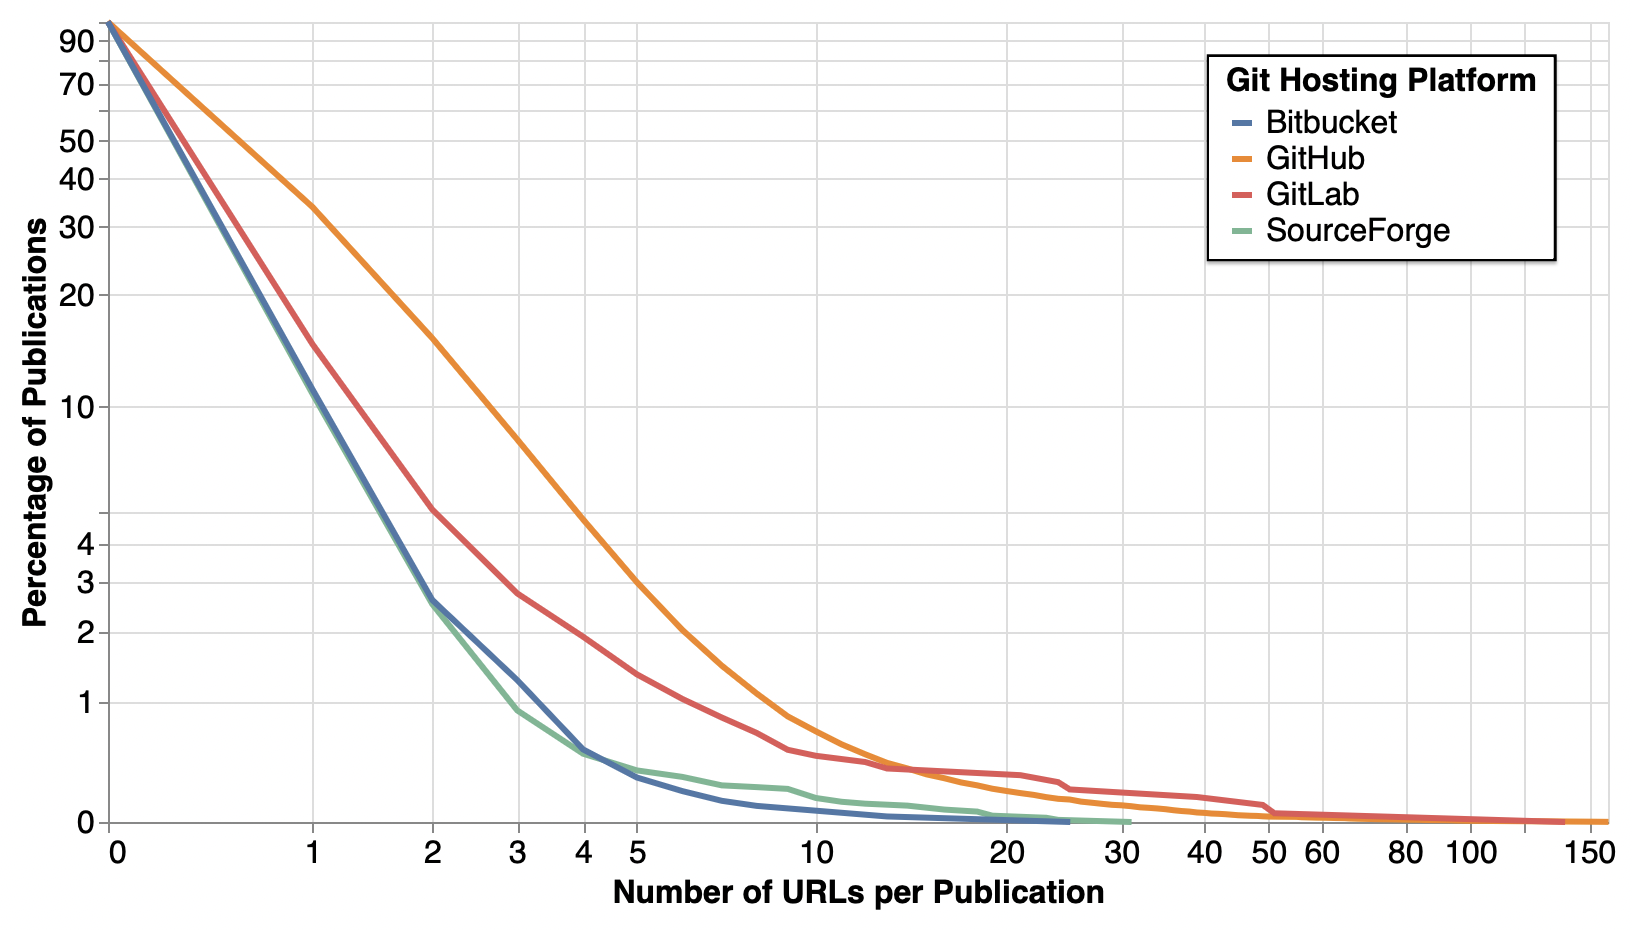
\includegraphics[width=\textwidth]{arxiv_ccdf.png}
    \caption{arXiv corpus}
    \label{fig:arxiv_ccdf}
\end{subfigure}
\hfill
\begin{subfigure}{\textwidth}
    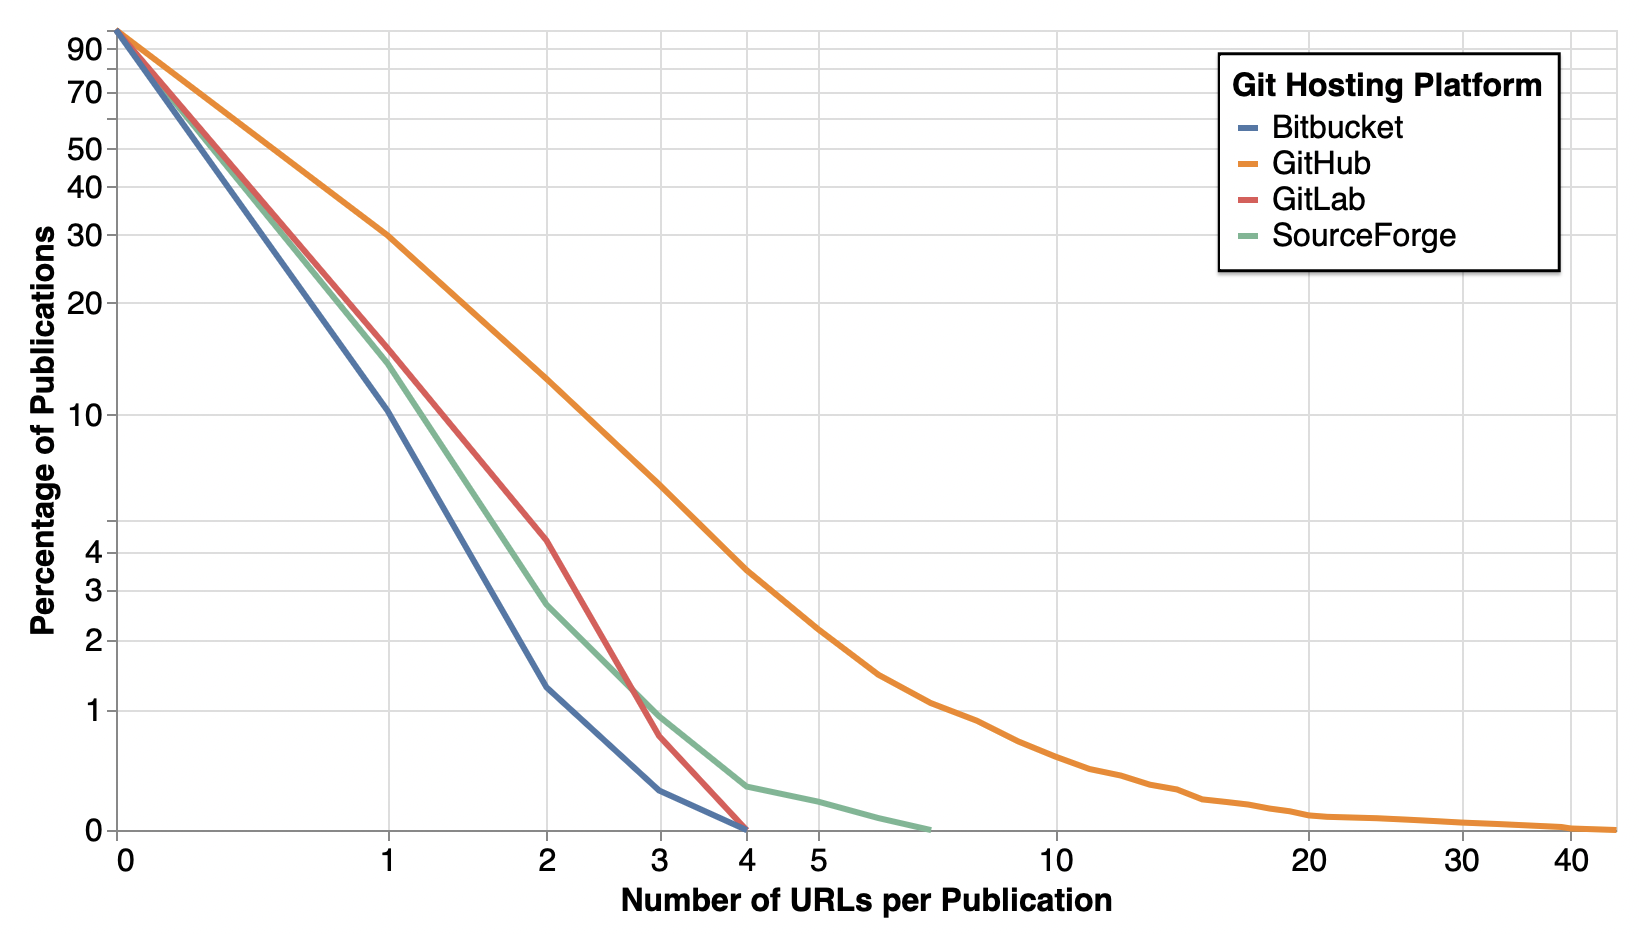
\includegraphics[width=\textwidth]{pmc_ccdf.png}
    \caption{PMC corpus}
    \label{fig:pmc_ccdf}
\end{subfigure}
        
\caption{If a publication links to GHP, how many links does it have? This figure is a Complementary Cumulative Distribution Function (CCDF) graphing the frequency of GHP URIs in publications with 1 or more GHP URI}
\label{fig:ccdf}
\end{figure}

Publications with multiple references to GitHub imply the repositories have significant value and relevance for the authors, indicating that they deemed the repository contents important to the content of the publication. As a result, these repositories should be preserved in archives to guarantee that future readers can access the publication's full context.

We also analyzed the use of URIs to GHPs by discipline for the arXiv corpus. When submitting an article to arXiv, authors are prompted to select the primary discipline of the article. We used the metadata associated with each article to map each discipline to the four GHPs based on the number of URIs to each GHP. Figure \ref{fig:chord_diagram} shows a visualization of the relationship between GHPs and STEM disciplines. Computer Science and Physics contain the highest number of URIs to a GHP. Considering the prevalence of software products and models in the Computer Science and Physics disciplines, these results are not surprising.

\begin{figure}
    \centering
    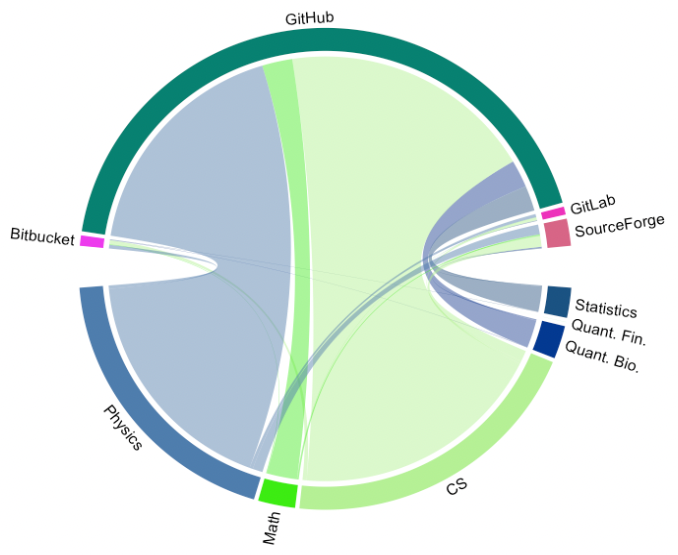
\includegraphics[width=\textwidth]{chord_diagram.png}
    \caption{Mapping the number of links to a GHP (top half of the diagram) by discipline (bottom half) for the arXiv corpus}
    \label{fig:chord_diagram}
\end{figure}